\chapter{Values and Functions}
\label{chap:let}
%
In this chapter, we will see how we can bind expressions to identifiers either as new constants, functions, or operators, how this saves time when building large programs, and how this makes programs easier to read and debug. As an example, consider the following problem,
\begin{problem}
  For given set constants $a$, $b$, and $c$, solve for $x$ in
  \begin{equation}
  a x^2+bx+c = 0
\end{equation}
\end{problem}
To solve for $x$ we use the quadratic formula from elementary algebra,
\begin{equation}
  x = \frac{-b\pm\sqrt{b^2-4ac}}{2a},
\end{equation}
which gives the general solution for any values of the coefficients. Here, we will assume a positive discriminant, $b^2-4ac>0$. In order to write a program where the code may be reused later, we define a function \mbox{\lstinline!discriminant : float -> float -> float -> float!}, that is, a function that takes 3 arguments, \lstinline!a!, \lstinline!b!, and \lstinline!c!, and calculates the discriminant. Likewise, we will define \mbox{\lstinline!positiveSolution : float -> float -> float -> float!} and \mbox{\lstinline!negativeSolution : float -> float -> float -> float!}, that also take the polynomial's coefficients as arguments and calculate the solution corresponding to choosing the positive and negative sign for $\pm$ in the equation. Details on function definition is given in \Cref{sec:functions}. Our solution thus looks like \Cref{identifiersExample}.
%
\fs{identifiersExample}{Finding roots for quadratic equations using function name binding.}
%
Here, we have further defined names of values \lstinline!a!, \lstinline!b!, and \lstinline!c! which are used as inputs to our functions, and the results of function application are bound to the names \lstinline!d!, \lstinline!xn!, and \lstinline!xp!. The names of functions and values given here are examples of identifiers, and with these, we may reuse the quadratic formulas and calculated values later, while avoiding possible typing mistakes and reducing the amount of code which needs to be debugged.

The use of identifiers is central in programming. For F\#, not to be confused with built-in functionality, identifiers must follow a specific set of rules: 
\begin{description} 
\item[Identifier]\idxs{identifier}~\\[-5mm]
  \begin{itemize}
  \item Identifiers are used as names for values, functions, types etc.
  \item They must start with a Unicode letter or underscore '\_', but can be followed by zero or more of letters, digits, and a range of special characters except for SP, LF, and CR (space, line feed, and carriage return). See \Cref{sec:unicode} for more on codepoints that represents letters. 
  \item They can also be a sequence of identifiers separated by a period.
  \item They cannot be keywords, see \Cref{tab:keywords}.
  \end{itemize}
\end{description}
\begin{table}
  \centering
  \rowcolors{2}{oddRowColor}{evenRowColor}
  \begin{tabularx}{\textwidth}{|l|>{\raggedright\arraybackslash}X|}
    \hline
    \rowcolor{headerRowColor} Type & Keyword\\
    \hline
  Regular 
  &\mbox{\lstinline{abstract},} \mbox{\lstinline{and},} \mbox{\lstinline{as},} \mbox{\lstinline{assert},} \mbox{\lstinline{base},} \mbox{\lstinline{begin},} \mbox{\lstinline{class},} \mbox{\lstinline{default},} \mbox{\lstinline{delegate},} \mbox{\lstinline{do},} \mbox{\lstinline{done},} \mbox{\lstinline{downcast},} \mbox{\lstinline{downto},} \mbox{\lstinline{elif},} \mbox{\lstinline{else},} \mbox{\lstinline{end},} \mbox{\lstinline{exception},} \mbox{\lstinline{extern},} \mbox{\lstinline{false},} \mbox{\lstinline{finally},} \mbox{\lstinline{for},} \mbox{\lstinline{fun},} \mbox{\lstinline{function},} \mbox{\lstinline{global},} \mbox{\lstinline{if},} \mbox{\lstinline{in},} \mbox{\lstinline{inherit},} \mbox{\lstinline{inline},} \mbox{\lstinline{interface},} \mbox{\lstinline{internal},} \mbox{\lstinline{lazy},} \mbox{\lstinline{let},} \mbox{\lstinline{match},} \mbox{\lstinline{member},} \mbox{\lstinline{module},} \mbox{\lstinline{mutable},} \mbox{\lstinline{namespace},} \mbox{\lstinline{new},} \mbox{\lstinline{null},} \mbox{\lstinline{of},} \mbox{\lstinline{open},} \mbox{\lstinline{or},} \mbox{\lstinline{override},} \mbox{\lstinline{private},} \mbox{\lstinline{public},} \mbox{\lstinline{rec},} \mbox{\lstinline{return},} \mbox{\lstinline{sig},} \mbox{\lstinline{static},} \mbox{\lstinline{struct},} \mbox{\lstinline{then},} \mbox{\lstinline{to},} \mbox{\lstinline{true},} \mbox{\lstinline{try},} \mbox{\lstinline{type},} \mbox{\lstinline{upcast},} \mbox{\lstinline{use},} \mbox{\lstinline{val},} \mbox{\lstinline{void},} \mbox{\lstinline{when},} \mbox{\lstinline{while},} \mbox{\lstinline{with},} and \mbox{\lstinline{yield}.}\\
 Reserved
 & \mbox{\lstinline{atomic},} \mbox{\lstinline{break},} \mbox{\lstinline{checked},} \mbox{\lstinline{component},} \mbox{\lstinline{const},} \mbox{\lstinline{constraint},} \mbox{\lstinline{constructor},} \mbox{\lstinline{continue},} \mbox{\lstinline{eager},} \mbox{\lstinline{fixed},} \mbox{\lstinline{fori},} \mbox{\lstinline{functor},} \mbox{\lstinline{include},} \mbox{\lstinline{measure},} \mbox{\lstinline{method},} \mbox{\lstinline{mixin},} \mbox{\lstinline{object},} \mbox{\lstinline{parallel},} \mbox{\lstinline{params},} \mbox{\lstinline{process},} \mbox{\lstinline{protected},} \mbox{\lstinline{pure},} \mbox{\lstinline{recursive},} \mbox{\lstinline{sealed},} \mbox{\lstinline{tailcall},} \mbox{\lstinline{trait},} \mbox{\lstinline{virtual},} and \mbox{\lstinline{volatile}.}\\
 Symbolic
 & \mbox{\lstinline{let!},} \mbox{\lstinline{use!},} \mbox{\lstinline{do!},} \mbox{\lstinline{yield!},} \mbox{\lstinline{return!},} \mbox{\lstinline{|},} \mbox{\lstinline{->},} \mbox{\lstinline{<-},} \mbox{\lstinline{.},} \mbox{\lstinline{:},} \mbox{\lstinline{(},} \mbox{\lstinline{)},} \mbox{\lstinline{[},} \mbox{\lstinline{]},} \mbox{\lstinline{[<},} \mbox{\lstinline{>]},} \mbox{\lstinline{[|},} \mbox{\lstinline{|]},} \mbox{\lstinline{\{},} \mbox{\lstinline{\}},} \mbox{\lstinline{'},} \mbox{\lstinline{#},} \mbox{\lstinline{:?>},} \mbox{\lstinline{:?},} \mbox{\lstinline{:>},} \mbox{\lstinline{..},} \mbox{\lstinline{::},} \mbox{\lstinline{:=},} \mbox{\lstinline{;;},} \mbox{\lstinline{;},} \mbox{\lstinline{=},} \mbox{\lstinline{_},} \mbox{\lstinline{?},} \mbox{\lstinline{??},} \mbox{\lstinline{(*)},} \mbox{\lstinline{<@},} \mbox{\lstinline{@>},} \mbox{\lstinline{<@@},} and \mbox{\lstinline{@@>}.} \\
 Reserved symbolic
 &\mbox{\lstinline{\~}} and \mbox{\lstinline{`}}\\
    \hline
  \end{tabularx}
  \caption{Table of (possibly future) \emph{keywords}\idxss{keyword} and symbolic keywords in F\#.}
  \label{tab:keywords}
\end{table}
Examples of identifiers are: \lstinline{a}, \lstinline{theCharacter9}, \lstinline{Next_Word}, \lstinline{_tok}, and \lstinline{f.sharp.rocks}.  Since programmers often work in multilingual environment dominated by the English language it is advicable to \advice{restrict identifiers to use letters from the English alphabet, numbers, period, and '\_'.}  However, the number of possible identifiers is enormous. The full definition refers to the Unicode general categories described in Appendix~\ref{sec:unicode}, and there are currently 19.345 possible Unicode code points in the letter category and 2.245 possible Unicode code points in the special character category.

Identifiers may be used to carry information about their intended content and use, and careful selection of identifiers can aid programmers to communicate thoughts about the code. Thus, identifiers are often a word or several concatenated words conveying some relevant meaning. For example, in the function definition \lstinline{let discriminant a b c = b ** 2.0 - 4.0 * a * c}, the function identifier has been chosen to be \lstinline{discriminant}. F\# places no special significance to the word 'discriminant', and the program would work exactly the same had the function been called \lstinline{let f a b c = b ** 2.0 - 4.0 * a * c}. However, to programmers, the word 'discriminant' informs us of the intended role of the function and thus is much preferred. This is a general principle: \advice{identifier names should be chosen to reflect their semantic value.}. The arguments \lstinline{a}, \lstinline{b}, and \lstinline{c} are short, but adheres to a textbook tradition of elementary algebra. Again, we might as well have used, \lstinline{let discriminant c a b = a ** 2.0 - 4.0 * c * b}, which is semantically identical to the original expression, but due to tradition, this would confuse most readers of the code. Thus, \advice{identifier names should be chosen consistently with the readers' traditions.} Finally, identifiers are often concatenations of words, as \lstinline{positiveSolution} in \Cref{identifiersExample}. Concatenations can be difficult to read. Without the capitalization of the second word, we would have had \lstinline{positivesolution}. This is readable at most times, but takes longer time to understand in general. Typical solutions are to use a separator, such as \lstinline{positive_solution}, \idx{lower camel case} also known as \idx{mixed case} as in the example \lstinline{positiveSolution}, and \idx{upper camel case} also known as \idx{pascal case} as \lstinline{PositiveSolution}. In this book, we use lower camel case except where F\# requires a capital first letter. Again, the choice does not influence what a program does, only how readable it is to a fellow programmer. The important part is that \advice{identifier names consisting of concatenated words are often preferred over names with few character, and concatenation should be emphasized, e.g., by camel casing.} Choosing the length of identifier names is a balancing act, since when working with large programs, very long identifier names can be tiresome to write, and a common practice is that the length of identifier names is proportional to the complexity of the program. I.e., complex programs use long names, simple programs use short names. What is complex and what is simple is naturally in the eye of the beholder, but when you program, remember that a future reader of the program most likely has not had time to work with the problem as long as the programmer, thus \advice{choose identifier names as if you were to explain the meaning of a program to a knowledgeable outsider.}

Another key concept in F\# is expressions. An expression can be a mathematical expression, such as $3*5$, a function application, such as $f 3$, and many other things. Central in this chapter is the binding of values and functions to identifiers, which is done with the keyword \keyword{let}, e.g., \lstinline!let a = 1.0!.

Expressions are the main workhorse of F\# and have an enormous variety in how they may be written. We will in this book gradually work through some of the more important facets.
\begin{description} 
\item[Expressions]\idxs{expression}~\\[-5mm]
  \begin{itemize}
  \item An Expression is a computation such as \lstinline{3 * 5}.
  \item They can be value bindings between identifiers and expressions that evaluate to a value or a function, see \Cref{sec:values,sec:functions}.
  \item They can be \lstinline{do}-bindings that produce side-effects and whose result are ignored, see \Cref{sec:functions} 
  \item They can be assignments to variables, see \Cref{sec:values}.
  \item They can be a sequence of expressions separated with the \idx[;@\lstinline{;}]{\lexeme{;}} lexeme.
  \item They can be annotated with a type by using the \idx[:@\lstinline{:}]{\lexeme{:}} lexeme.
  \end{itemize}
\end{description}

Before we begin a deeper discussion on bindings, note that F\#  adheres to two different syntaxes: \idx[verbose syntax]{verbose} and \idx[lightweight syntax]{lightweight}. In the verbose syntax, newlines and whitespaces are generally ignored, while in lightweight syntax, certain keywords and lexemes may be replaced by newlines and whitespaces. The lightweight syntax is the most common, but the syntaxes may be mixed, and we will highlight the options, when relevant.

\section{Value Bindings}
\label{sec:values}
Binding identifiers to literals, or expressions that are evaluated to be values, is called \idx{value-binding}, and examples are \lstinline!let a = 3.0! and \lstinline!let b = cos 0.9!. Value bindings have the following syntax:
%
\begin{verbatimwrite}{\ebnf/valueBindings.ebnf}
let <*valueIdent*> = <*bodyExpr*> [*in <*expr*>*]
\end{verbatimwrite}
\syntax{\ebnf/valueBindings.ebnf}{Value binding expression.}
%
The \idx[let@\lstinline{let}]{\keyword{let}} keyword binds a value-identifier \lstinline[language=syntax]{<*valueIdent*>} with an expression \lstinline[language=syntax]{<*bodyExpr*>} that evaluates to a value. The following square bracket notation \lstinline[language=syntax]{[**]} means that the enclosed is optional, and F\# is able to identify whether or not the optional part is used by whether or not the \idx[in@\lstinline{in}]{\keyword{in}} keyword is present in the binding expression. If the \keyword{in} keyword is used, then the value-identifier is a local definition in the following \lstinline[language=syntax]{<*expr*>} expression but in the following lines. For lightweight syntax, the \keyword{in} keyword is replaced with a newline, and the binding \emph{is} valid in the following lines at the level of scope of the value-binding, or deeper, lexically.

The value identifier annotated with a type by using the \idx[:@\lstinline{:}]{\lexeme{:}} lexeme followed by the name of a type, e.g., \lstinline{int}. The \idx[\_@\lstinline{_}]{\lexeme{\_}} lexeme may be used as a value-identifier. This lexeme is called the \idx{wildcard pattern}, and for value-bindings it means that \lstinline[language=syntax]{<*bodyExpr*>} is evaluated, but the result is discarded. See \Cref{chap:patterns} for more details on patterns.

For example, letting the identifier \lstinline!p! be bound to the value \lstinline!2.0! and using it in an expression is done as shown in \Cref{letValue}.
%
\fs{letValue}{The identifier \lstinline!p! is used in the expression following the \keyword{in} keyword.}
%
F\# will ignore most newlines between lexemes, i.e., the above is equivalent to writing as shown in \Cref{letValueLF}.
%
\fs{letValueLF}{Newlines after \keyword{in} make the program easier to read.}
%
F\# also allows for an alternative notation called \idx{lightweight syntax}, where e.g., the \keyword{in} keyword is replaced with a newline, and the expression starts on the next line at the same column as \keyword{let} starts in, i.e., the above is equivalent to \Cref{letValueLightWeight}.
%
\fs{letValueLightWeight}{Lightweight syntax does not require the \keyword{in} keyword, but the expression must be aligned with the \keyword{let} keyword.}
%
The same expression in interactive mode will also show with the inferred types, as shown in \Cref{letValueLightWeightTypes}.
%
\fsOutput{letValueLightWeightTypes}{Interactive mode also outputs inferred types.}
%
By the \keyword{val} keyword in the line \lstinline!val p : float = 2.0!, we see that \lstinline!p! is inferred to be of type \lstinline!float! and bound to the value \lstinline!2.0!. The inference is based on the type of the right-hand-side which is \lstinline!float!.  Identifiers may be defined to have a type using the \lexeme{:} lexeme, but the types on the left-hand-side and right-hand-side of the \lexeme{=} lexeme must be identical. Mixing types gives an error, as shown in \Cref{letValueTypeError}.
%
\fs{letValueTypeError}{Binding error due to type mismatch.}
% \begin{lstlisting}[language=fsharp,caption={fsharpi, binding error due to type mismatch.}]
%   > let a : float = 3;;
%
%   let a : float = 3;;
%   ----------------^
%
% /Users/sporring/repositories/fsharpNotes/stdin(50,17): error FS0001: This expression was expected to have type
%     float    
% but here has type
%     int    
% \end{lstlisting}
Here, the left-hand-side is defined to be an identifier of type float, while the right-hand-side is a literal of type integer.

An expression can be a sequence of expressions separated by the lexeme \lexeme{;}, see \Cref{letValueSequence}.
%
\fs{letValueSequence}{A value-binding for a sequence of expressions.}
%
The lightweight syntax automatically inserts the \lexeme{;} lexeme at newlines, hence using the lightweight syntax, the above is the same as shown in \Cref{letValueSequenceLightWeight}.
%
\fs{letValueSequenceLightWeight}{A value-binding for a sequence using lightweight syntax.}
%

A key concept of programming is \idx{scope}. When F\# seeks the value bound to a name, it looks left and upward in the program text for its \keyword{let}-binding in the present or higher scopes, see \Cref{letValueScopeLower} for an example. This is called \idx{lexical scope}.
%
\fs{letValueScopeLower}{Redefining identifiers is allowed in lower scopes.}
%
Some special bindings are mutable, in which case F\# uses the \idx{dynamic scope}, that is, the value of a binding is defined by when it is used. This will be discussed in \Cref{sec:mutableValues}.

Scopes are given levels, and scopes may be nested, where the nested scope has a level one lower than its parent.\jon{Drawings would be good to describe scope} F\# distinguishes between the top and lower levels, and at the top level in the lightweight syntax, redefining values is not allowed, as shown in \Cref{letValueScopeLowerError}.
%
\fs{letValueScopeLowerError}{Redefining identifiers is not allowed in lightweight syntax at top level.}
%
%But using \keyword{begin} and \keyword{end} keywords, we create a \idx{block} which acts as a \idx{nested scope}, and then redefining is allowed, e.g.,
% %
% \fs{letValueScopeBlockAlternative2}{A block has lower scope level, and rebinding is allowed.}
% %
% It is said that the second binding \idx{overshadows} the first.
% Alternatively, we may use parentheses to create a block, e.g.,
However, using parentheses, we create a \idx{code block}, i.e., a \idx{nested scope}, and then redefining is allowed, as demonstrated in \Cref{letValueScopeBlockAlternative3}.
%
\fs{letValueScopeBlockAlternative3}{A block may be created using parentheses.}
%
Nevertheless, \advice{avoid reusing names unless it's in a deeper scope.}

Inside the block in \Cref{letValueScopeBlockAlternative3} we used indentation, which is good practice, but not required here.

Bindings inside a nested scope are not available outside, as shown in \Cref{letValueScopeNestedScope}.
%
\fs{letValueScopeNestedScope}{Bindings inside a scope are not available outside.}
%
Nesting is a natural part of structuring code, e.g., through function definitions to be discussed in \Cref{sec:functions} and flow control structures to be discussed in \Cref{chap:flow}. Blocking code by nesting is a key concept for making robust code that is easy to use by others, without the user necessarily needing to know the details of the inner workings of a block of code.

Defining blocks is used for controlling the extent of a lexical scope of bindings. For example, adding a second \lstinline!printfn! statement, as in \Cref{letValueScopeBlockProblem},
will print the value 4, last bound to the identifier \lstinline!p!, since F\# interprets the above as \lstinline!let p = 3 in let p = 4 in (printfn "%A" p; printfn "%A" p)!. %
%
\fs{letValueScopeBlockProblem}{Overshadowing hides the first binding.}
%
Had we intended to print the two different values of \lstinline!p!, then we should have created a block as in \Cref{letValueScopeBlock}.
%
\fs{letValueScopeBlock}{Blocks allow for the return to the previous scope.}
%
%Here, the lexical scope of \lstinline!let p = 4! is for the nested scope, which ends at \lexeme{)}, returning to the lexical scope of \lstinline!let p = 3 in ...!. %Alternatively, the \keyword{begin} and \keyword{end} keywords could equally have been used.
%\fs{letValueScopeBlockAlternative}{}

\section{Function Bindings}
\label{sec:functions}
A function is a mapping between an input and output domain. A key advantage of using functions when programming is that they encapsulate\idxss{encapsulation} code into smaller units, that are easier to debug and may be reused. F\# is a functional first programming language and offers a number of alternative methods for specifying parameters, which will be discussed in this section. Binding identifiers to functions follows a syntax similar to value-binding,
%
\begin{verbatimwrite}{\ebnf/functionBindings.ebnf}
let <*funcIdent*> <*arg*> {*<*arg*>*} |* () = <*bodyExpr*> [*in <*expr*>*]
\end{verbatimwrite}
\syntax{\ebnf/functionBindings.ebnf}{Function binding expression}
%
Here \lstinline[language=syntax]{<*funcIdent*>} is an identifier and is the name of the function, \lstinline[language=syntax]{<*arg*>} is zero or more identifiers, that bind to the value used when calling the function, and which is to be used in the body of the function, the expression \lstinline[language=syntax]{<*bodyExpr*>}. The \lstinline[language=syntax]{|*} notation denotes a choice, i.e., either that on the left-hand-side or that on the right-hand-side. Thus \lstinline{let f x = x * x} and \lstinline{let f () = 3} are valid function bindings, but \lstinline{let f = 3} would be a value binding, not a function binding. The arguments and the function may be annotated with a type, in which case for arguments we write
%
\begin{verbatimwrite}{\ebnf/functionBindingsAnnotated.ebnf}
let <*funcIdent*> (<*arg*> : <*type*>) {*(<*arg*> : <*type*>)*} : <*type*> |* () : <*type*> = <*bodyExpr*> [*in <*expr*>*]
\end{verbatimwrite}
\syntax{\ebnf/functionBindingsAnnotated.ebnf}{Function binding expression}
%
where \lstinline[language=syntax]{<*type*>} is a name of an existing type. The argument types are given in parentheses, and the return type is given last. 

Functions are a key concept in F\#, and in this chapter we will discuss the very basics. Recursive functions will be discussed in \Cref{chap:flow} and higher-order functions in \Cref{chap:higherOrderFunctions}.

An example of defining a function and using it in interactive mode is shown in \Cref{letFunction}.
%
\fsOutput{letFunction}{An example of a binding of an identifier and a function.}
%
Here we see that the function is interpreted to have the type \lstinline!val sum : x:float -> y:float -> float!. The \lexeme{->} lexeme means a mapping between sets, in this case, floats. The function is also a higher-order function, to be discussed in detail below, and here it suffices to think of \lstinline!sum! as a function that takes 2 floats as argument and returns a float.
%, that \lexeme{->} associates to the right, hence \lstinline!x:float -> y:float -> float! is equivalent to \lstinline!x:float -> (y:float -> float)! and thus, \lstinline!sum x! is a function, which gives a function

Not all types need to be declared, just a sufficient number for F\# to be able to infer the types for the full statement. For the example, one is sufficient, and we could just have declare the type of the result, as in \Cref{letFunctionAlterantive}.
%
\fsCode{letFunctionAlterantive}{letFunctionAlterantive}{Not every type needs to be declared.}{}
%
Or even just one of the arguments, as in \Cref{letFunctionAlterantive2}.
%
\fsCode{letFunctionAlterantive2}{letFunctionAlterantive2}{Just one type is often enough for F\# to infer the rest.}{}
%
In both cases, since the \lstinline|+| \idx{operator} is only defined for \idx[operand]{operands} of the same type, declaring the type of either arguments or result implies the type of the remainder.  As for values, lightweight syntax automatically inserts the keyword \keyword{in} and the lexeme \lexeme{;}, as shown in \Cref{letFunctionLightWeight}.
%
\fs{letFunctionLightWeight}{Lightweight syntax for function definitions.}
%

Arguments need not always be inferred to types, but may be of the generic type when \idx{type safety} is ensured, as shown in \Cref{functionDeclarationGeneric}.
%
\fsOutput{functionDeclarationGeneric}{Type safety implies that a function will work for any type.}
%
Here, the function \lstinline{second} does not use the first argument \lstinline{x}, which therefore can be of any type, and which F\#, therefore, calls \lstinline{'a}. The type of the second element, \lstinline{y}, can also be of any type and not necessarily the same as \lstinline!x!, so it is called \lstinline!'b!. Finally, the result is the same type as \lstinline!y!, whatever it is. This is an example of a \idx{generic function}, since it will work on any type.

A function may contain a sequence of expressions but must return a value. E.g., the quadratic formula may be written as shown in \Cref{identifiersExampleAdvance}. 
%
\fs{identifiersExampleAdvance}{A function may contain sequences of expressions.}
%
Here, we used the lightweight syntax, where the \lexeme{=} identifies the start of a nested scope, and F\# identifies the scope by indentation. The amount of space used for indentation does not matter, but all lines in the same scope must use the same amount. The scope ends before the first line with the previous indentation or none. Notice how the last expression is not bound to an identifier, but is the result of the function, i.e., in contrast to many other languages, F\# does not have an explicit keyword for returning values, but requires a final expression, which will be returned to the caller of the function. Note also that since the function \lstinline!discriminant! is defined in the nested scope of \lstinline!solution!, and becausethe scope ends before \lstinline!let a = 1.0!, \lstinline!discriminant! cannot be called outside \lstinline!solution!.

\idx[lexical scope]{Lexical scope} and function definitions can be a cause of confusion, as the following example in \Cref{lexicalScopeNFunction} shows.\jon{Add a drawing or possibly a spell-out of lexical scope here.}
%
\fs{lexicalScopeNFunction}{Lexical scope means that $f(z) = 3x$ and not $4x$ at the time of calling.}
%
Here, the value-binding for \lstinline!a! is redefined after it has been used to define a helper function \lstinline!f!. So which value of \lstinline!a! is used when we later apply \lstinline!f! to an argument? To resolve the confusion, remember that value-binding is lexically defined, i.e., the binding \lstinline!let f z = a * z! uses the value of \lstinline!a! as it is defined by the ordering of the lines in the script, not dynamically by when \lstinline!f! was called. Hence, \advice{think of lexical scope as substitution of an identifier with its value or function immediately at the place of definition.} Since \lstinline!a! and \lstinline!3.0! are synonymous in the first lines of the program, the function \lstinline!f! is really defined as \lstinline!let f z = 3.0 * z!.

Functions do not need a name, but may be declared as an \idx[anonymous functions]{anonymous function} using the \idx[fun@\lstinline{fun}]{\keyword{fun}} keyword and the \idx[->@\lstinline{->}]{\lexeme{->}} lexeme, as shown in \Cref{functionDeclarationAnonymous}.
%
\fs{functionDeclarationAnonymous}{Anonymous functions are functions as values.}
%
Here, a name is bound to an anonymous function which returns the first of two arguments. The difference to \lstinline!let first x y = x! is that anonymous functions may be treated as values, meaning that they may be used as arguments to other functions and the new values may be reassigned to their identifiers when mutable, as will be discussed in \Cref{sec:mutableValues}. A common use of anonymous functions is as arguments to other functions, as demonstrated in \Cref{functionDeclarationAnonymousAdvanced}.
%
\fs{functionDeclarationAnonymousAdvanced}{Anonymous functions are often used as arguments for other functions.}
%
Note that here \lstinline!apply! is given 3 arguments: the function \lstinline!mul! and 2 integers. It is not given the result of \lstinline!mul 3 6!, since that would not match the definition of \lstinline!apply!. \advice{Anonymous functions and functions as arguments are powerful concepts, but tend to make programs harder to read, and their use should be limited.}

The result of one function is often used as an argument of another. This is function composition, and an example is shown in \Cref{functionComposition}.
%
\fs{functionComposition}{Composing functions using intermediate bindings.}
%
In the example we combine two functions \lstinline{f} and \lstinline{g} by storing the result of \lstinline{f 2} in \lstinline{a} and using that as argument of \lstinline{g}. This is the same as \lstinline{g (f 2)}, and in the later case, the compile creates a temporary value for \lstinline{f 2}. Such compositions are so common in F\# that a special set of operators has been invented, called the \idx{piping} operators: \idx[{|>}@\lstinline{|>}]{\lexeme{|>}} and \idx[{<|}@\lstinline{<|}]{\lexeme{<|}}. They are used as demonstrated in \Cref{functionPiping}.
%
\fs{functionPiping}{Composing functions by piping.}
%
The example shows regular composition, left-to-right, and right-to-left piping. The word piping is a picturial description of data as if it were flowing through pipes, where functions are connection points of pipes distributing data in a network. The three expressions in \Cref{functionPiping} perform the same calculation. The left-to-right piping in line~\ref{functionPipingLeftToRight} corresponds to the left-to-right reading direction, i.e., the value \lstinline{2} is used as argument to \lstinline{f}, and the result is used as argument to \lstinline{g}. In contrast, right-to-left piping in line~\ref{functionPipingRightToLeft} has the order of arithmetic composition as line~\ref{functionPipingComposition}. Unfortunately, since the piping operators are left-associatitve, without the parenthesis in line~\ref{functionPipingRightToLeft} \mbox{\lstinline{g <| f <| 2}}, F\# would read the expression as \lstinline{(g <| f) <| 2}. That would have been an error, since \lstinline{g} takes an integer as argument, not a function. F\# can also define composition on a function level. Further discussion on this is deferred to \Cref{chap:higherOrderFunctions}. The piping operator comes in four variants: \lexeme{||>}, \lexeme{<||}, \lexeme{|||>}, and \lexeme{<|||}. These allow for piping between pairs and triples to functions of 2 and 3 arguments, see \Cref{functionTuplePiping} for an example.
%
\fs{functionTuplePiping}{Tuples can be piped to functions of more than one argument.}
%
The example demonstrates right-to-left piping, left-to-right works analogously.\jon{Tuples have not yet been introduced!}

A \idx{procedure} is a generalization of the concept of functions, and in contrast to functions, procedures need not return values. This is demonstrated in \Cref{procedure}.
%
\fs{procedure}{A procedure is a function that has no return value, and in F\# returns \lexeme{()}.}
%
In F\#, this is automatically given the unit type as the return value. Procedural thinking is useful for \idx{encapsulation} of scripts, but is prone to \idx[side-effect]{side-effects}. 
%An example, we've already seen is the \lstinline{printfn}, which is used to print text on the console, but does not return a value. Coincidentally, since the console is a state, printing to it is a side-effect. Above we examined 
%\begin{fse}
%   let updateFactor factor = 
%    factor := 2
%\end{fse}
%\fsCode{mutableAssignReturnSideEffectStump}{mutableAssignReturnSideEffectStump}{}{}
%which also does not have a return value. 
For this reason, it is adviced to \advice{prefer functions over procedures.}  More on side-effects in \Cref{sec:mutableValues}.

In F\#, functions (and procedures) are \idx[first-class citizenship]{first-class citizens}, which means that functions are values: They may be passed as arguments, returned from a function, and bound to a name. For first-class citizens, the name it is bound to does not carry significance to the language, as, e.g., illustrated with the use of anonymous functions. Technically, a function is stored as a \idx{closure}. A closure is a description of the function, its arguments, its expression, and the environment at the time it was created, i.e., the triple $(args, exp, env)$. Consider the listing in \Cref{functionFirstClass}.
%
\fs{functionFirstClass}{The function \lstinline{ApplyFactor} has a non-trivial closure.}
%
It defines two functions \lstinline{mul} and \lstinline{applyFactor}, where the latter is a higher-order function taking another function as an argument and uses part of the environment to produce its result. The two closures are:
\begin{align}
  \text{\lstinline{mul}}: \left(\text{args}, \text{exp}, \text{env}\right) 
  = &\big((\text{\lstinline{x}},\text{\lstinline{y}}), \left(\text{\lstinline{x * y}}\right), ()\big)
  \\\text{\lstinline{applyFactor}}: \left(\text{args}, \text{exp}, \text{env}\right) 
  = &\left((\text{\lstinline{x}}, \text{\lstinline{fct}}), \left(\begin{subarray}{l}\displaystyle\text{\lstinline{let a = fct factor x}}\\\displaystyle\text{\lstinline{string a}}\end{subarray}\right),\left(\text{\lstinline{factor}} \rightarrow 2.0\right)\right)
\end{align}
The function \lstinline{mul} does not use its environment, and everything needed to evaluate its expression are values for its arguments. The function \lstinline{applyFactor} also takes two arguments, a function and a value. It uses \lstinline{factor} from the environment, thus this is stored in its closure. When \lstinline{mul} is given as an argument in \Cref{functionFirstClass} line~\ref{functionFirstClassApplyFactor}, then it is its closure which is given to \lstinline{applyFactor}, and the closure contains everything that \lstinline{applyFactor} requires to use \lstinline{mul}. Likewise, if \lstinline{applyFactor} is given as argument to yet another function, then its closure includes the relevant part of its environment at the time of definition, \lstinline{factor}, such that when \lstinline{applyFactor} is applied to two arguments, then its closure contains everything needed to evaluate its expression.

\section{Operators}
\label{sec:operators}
Operators are functions, and in F\#, the infix multiplication operator \lstinline!+! is equivalent to the function \lstinline!(+)!, as shown in \Cref{addOperatorNFunction}.
%
\fs{addOperatorNFunction}{Operators have function equivalents.}
%
All operators have this option, and you may redefine them and define your own operators, but in F\# names of user-defined operators are limited:
\begin{itemize}
\item A \idx{unary operator} name can be: \lexeme{+}, \lexeme{-}, \lexeme{+.}, \lexeme{-.}, \lexeme{\%}, \lexeme{\&}, \lexeme{\&\&}, \lexeme{\~\~}, \lexeme{\~\~\~}, \lexeme{\~\~\~\~}, \dots, apostropheOp. Here apostropheOp is an operator name starting with \lexeme{!} and followed by one or more of either \lexeme{!}, \lexeme{\%}, \lexeme{\&}, \lexeme{*}, \lexeme{+}, \lexeme{-}, \lexeme{.}, \lexeme{/}, \lexeme{<}, \lexeme{=}, \lexeme{>}, \lexeme{@}, \lexeme{^}, \lexeme{|}, \lexeme{\~}, but apostropheOp cannot be \lexeme{!=}.
\item An \idx{binary operator} name can be: \lexeme{+}, \lexeme{-}, \lexeme{+.}, \lexeme{-.}, \lexeme{\%}, \lexeme{\&}, \lexeme{\&\&}, \lexeme{:=}, \lexeme{::}, \lexeme{\$}, \lexeme{?}, dotOp. Here dotOp is an operator name starting with \lexeme{.} and followed by \lexeme{+}, \lexeme{-}, \lexeme{+.}, \lexeme{-.}, \lexeme{\%}, \lexeme{\&}, \lexeme{\&\&}, \lexeme{-}, \lexeme{+}, \lexeme{\|\|}, \lexeme{<}, \lexeme{>}, \lexeme{=}, \lexeme{\|}, \lexeme{\&}, \lexeme{\^}, \lexeme{*}, \lexeme{/}, \lexeme{\%}, \lexeme{!=}. Only \lexeme{?} and \lexeme{?<-} may start with \lexeme{?}.
  \end{itemize}
  The precedence rules and associativity of user-defined operators follow the rules for which they share prefixes with built-in rules, see \Cref{tab:someOperatorPrecedences}.
For example, \lstinline!.*!, \lstinline!+++!, and \lstinline!<+! are valid operator names for infix operators, they have precedence as ordered, and their associativities are all left. Using \lstinline!~! as the first character in the definition of an operator makes the operator unary and will not be part of the name. Examples of definitions and use of operators are,
%
\fs{operatorDefinitions}{Operators may be (re)defined by their function equivalent.}
%
Operators beginning with \lstinline!*! must use a space in its definition. For example, without a space \lstinline!( *! would be confused with the beginning of a comment \lstinline!(*!, see \Cref{chap:documentation} for more on comments in the code.

Beware, redefining existing operators lexically redefines all future uses of the operators for all types, hence \advice{it is not a good idea to redefine operators, but better to define new ones.}\spec{It seems there is a bug in mono: \lstinline{let (~+) x = x+1 in printfn "\%A" +1;;} prints 1 and not 2.} In \Cref{chap:oop} we will discuss how to define type-specific operators, including prefix operators. 

\section{Do-Bindings}
Aside from \keyword{let}-bindings that binds names with values or functions, sometimes we just need to execute code. This is called a \idx[do@\lstinline{do}]{\keyword{do}}-binding\idxs{do-binding} or, alternatively, a \idx{statement}. The syntax is as follows:
%
\begin{verbatimwrite}{\ebnf/doBindings.ebnf}
[*do *]<*expr*>
\end{verbatimwrite}
\syntax{\ebnf/doBindings.ebnf}{Syntax for \keyword{do}-bindings.}
%
The expression \lstinline[language=syntax]{<*expr*>} must return \keyword{unit}. The keyword \keyword{do} is optional in most cases, but using it emphasizes that the expression is not a function that returns a useful value. Procedures are examples of such expressions, and a very useful family of procedures are the \lstinline{printf} family described below. In the remainder of this book, we will refrain from using the \keyword{do} keyword.

\section{The Printf Function}
\label{sec:printf}
A common way to output information to the console is to use one of the family of \idx[printf@\lstinline{printf}]{\lstinline{printf}} commands. These functions are special, since they take a variable number of arguments, and the number is decided by the first argument - the format string. The syntax for the \lstinline{printf} commands are as follows:
%
\begin{verbatimwrite}{\ebnf/printf.ebnf}
printf <*format-string*> {*<*ident*>*}
\end{verbatimwrite}
\syntax{\ebnf/printf.ebnf}{\lstinline{printf} statement.}
%
The \lstinline[language=ebnf]!formatString! is a string (simple or verbatim) with placeholders. The function \lstinline[language=ebnf]!printf! prints \lstinline[language=ebnf]!formatString! to the console, where all \lstinline[language=ebnf]!placeholder! have been replaced by the values of the corresponding arguments formatted as specified. For example, in \mbox{\lstinline!printfn "1 2 \%d" 3!}, the \lstinline[language=ebnf]!formatString! is \mbox{\lstinline!"1 2 \%d"!} and the placeholder is \lstinline!%d!. %
When executed, \lstinline{printf} will replace \lstinline!%d! %
with the following argument, \lstinline{3}, and print the result to the console: \mbox{\lstinline!1 2 3!}.  There are specifiers for all the basic types, and more, as elaborated in \Cref{tab:printfPlaceholder}.
% 
\begin{table}
  \centering
  \rowcolors{2}{oddRowColor}{evenRowColor}
  \begin{tabularx}{\linewidth}{|l|l|X|}
    \hline
    \rowcolor{headerRowColor} Specifier& Type&Comment\\
    \hline
    \lstinline!\%b!&\lstinline!bool!&formatted as ``true'' or ``false''\\
    \hline
    \lstinline!\%s!&\lstinline!string!&\\
    \hline
    \lstinline!\%c!&\lstinline!char!&\\
    \hline
    \mbox{\lstinline!\%d!,} \mbox{\lstinline!\%i!}&basic integer&\\
    \hline
    \lstinline!\%u!&basic unsigned integers&\\
    \hline
    \lstinline!\%x!&basic integer&formatted as unsigned hexadecimal with lower case letters\\
    \hline
    \lstinline!\%X!&basic integer&formatted as unsigned hexadecimal with upper case letters\\
    \hline
    \lstinline!\%o!&basic integer&formatted as unsigned octal integer\\
    \hline
    \mbox{\lstinline!\%f!,} \mbox{\lstinline!\%F!,} &basic floats&formatted on decimal form\\
    \hline
    \mbox{\lstinline!\%e!,} \mbox{\lstinline!\%E!,} &basic floats&formatted on scientific form. Lower case uses "e" while upper case uses "E'' in the formatting.\\
    \hline
    \mbox{\lstinline!\%g!,} \mbox{\lstinline!\%G!,} &basic floats&formatted on the shortest of the corresponding decimal or scientific form.\\
    \hline
%    \lstinline!\%M!&decimal&\\
%    \hline
    \lstinline!\%A!, \lstinline!\%O!&any value&formatted as a basic type or using the object's \lstinline!ToString! method\\
    \hline
%    \lstinline!\%A!&any value&formatted as a basic type or using its \lstinline!ToString! method\\
%    \hline
%    \lstinline!\%a!&\lstinline[language=ebnf]!Printf.TextWriterFormat ->'a -> ()!&\\
%    \hline
%    \lstinline!\%t!&\lstinline[language=ebnf]!(Printf.TextWriterFormat -> ()!&\\
%    \hline
  \end{tabularx}
  \caption{Some printf placeholder strings.}
  \label{tab:printfPlaceholder}
\end{table}
The placeholder can be parametrized, e.g.,  the placeholder string \lstinline{%8s} %
will print a right-aligned string which that is eight characters wide and padded with spaces, as needed. For floating point numbers, \lstinline{%8f} %
will print a number that is exactly seven digits and a decimal point, making eight characters in total. Zeros are added after the decimal point, as needed. Alternatively, we may specify the number of digits after the decimal point, such that \lstinline{%8.1f} %
will print a floating point number, aligned to the right, with one digit after the decimal point padded with spaces, as needed. The default is for the value to be right justified in the field, but left justification can be specified by the \lstinline!-! character. For number types, you can specify their format by \lstinline!"0"! for padding the number with zeros to the left when right justifying the number; \lstinline!"+"! to explicitly show a plus sign for positive numbers; \lstinline!SP! to enforce a space, where there otherwise would be a plus sign for positive numbers. The placeholder parameter may also be given as an argument to \lstinline{printf} which case the placeholder should use the \lstinline!*! character instead of an integer.

Examples of placeholder parametrization are shown in \Cref{printfExample}.
%
\fs{printfExample}{Examples of printf and some of its formatting options.}
%
Not all combinations of flags and identifier types are supported, e.g., strings cannot have the number of integers after the decimal point specified.\spec{Mono seems to have a bug, \lstinline{printfn "\%.1g"   3.13;;} and \lstinline{printfn "\%.1f"   3.13;;} produces different number of digits.}\spec{Spec-4.0 \lstinline{\%s} and \lstinline{\%b} are missing in Section 3.1.16.}
The placeholder types \lstinline{"%A"}, %
\lstinline{"%a"}, %
and \lstinline{"%t"} %
are special for F\#, examples of their use are shown in \Cref{printfExampleAdvance}.
%
\fs{printfExampleAdvance}{Custom format functions may be used to specialise output.}
%
The \lstinline!%A! %
is special in that all built-in types, including tuples, lists, and arrays to be discussed in \Cref{chap:lists}, can be printed using this formatting string, but notice that the formatting performed includes the named literal string. The two formatting strings \lstinline!%t! %
and \lstinline!%a! %
are options for user-customizing the formatting and will not be discussed further.

Beware, \lstinline[language=ebnf]!formatString! is not a \lstinline!string! but a \lstinline!Printf.TextWriterFormat!, so to predefine a \lstinline[language=ebnf]!formatString! as, e.g., \mbox{\lstinline{let str = "hello \%s" in printf str "world"}}, will be a type error.

The family of \lstinline!printf! is shown in \Cref{tab:printfFamily}.\idxss{stdout@\lstinline{stdout}}\idxss{stderr@\lstinline{stderr}}\idxss{printf@\lstinline{printf}}\idxss{printfn@\lstinline{printfn}}\idxss{fprintf@\lstinline{fprintf}}\idxss{fprintfn@\lstinline{fprintfn}}\idxss{eprintf@\lstinline{eprintf}}\idxss{eprintfn@\lstinline{eprintfn}}\idxss{sprintf@\lstinline{sprintf}}\idxss{failwith@\lstinline{failwithf}}
\begin{table}
  \centering
  \rowcolors{2}{oddRowColor}{evenRowColor}
  \begin{tabularx}{\linewidth}{|l|l|X|}
    \hline
    \rowcolor{headerRowColor} Function & Example & Description\\
    \hline
    \lstinline!printf! & \lstinline!printf "\%d apples" 3! & Prints to the console, i.e., \lstinline!stdout!\\
    \lstinline!printfn! &  & As \lstinline!printf! and adds a newline.\\
    \hline
    \lstinline!fprintf! & \lstinline!fprintf stream "\%d apples" 3! & Prints to a stream, e.g., \lstinline!stderr! and \lstinline!stdout!, which would be the same as \lstinline!printf! and \lstinline!eprintf!.\\
    \lstinline!fprintfn! & & As \lstinline!fprintf! but with added newline.\\
    \hline
    \lstinline!eprintf! & \lstinline!eprintf "\%d apples" 3! & Prints to \lstinline!stderr!\\
    \lstinline!eprintfn! & & As \lstinline!eprintf! but with added newline.\\
    \hline
    \lstinline!sprintf! & \lstinline!printf "\%d apples" 3! & Return printed string\\
    \hline
    \lstinline!failwithf! & \lstinline!failwithf "\%d failed apples" 3! & Prints to a string and used for raising an exception.\\
    \hline
  \end{tabularx}
  \caption{The family of printf functions.}
  \label{tab:printfFamily}
\end{table}
The function \lstinline!fprintf! prints to a stream, e.g., \lstinline!stderr! and \lstinline!stdout!, of type \lstinline!System.IO.TextWriter!. For the moment it is sufficient to think of both \lstinline!stderr! and \lstinline!stdout! to be the console. Streams will be discussed in further detail in \Cref{chap:IO}. The function \lstinline!failwithf! is used with exceptions, see \Cref{chap:errors} for more details. The function has a number of possible return value types, and for testing, the \idx[ignore@\lstinline{ignore}]{\lstinline{ignore}} function ignores it all, e.g., \mbox{\lstinline!ignore (failwithf "\%d failed apples" 3)!}.
\spec{Mono: \lstinline{bprintf} and \lstinline{kprintf} are undefined.}

\section{Reading from the Console}
\label{sec:readline}
The \lstinline{printf} and \lstinline{printfn} functions allow us to write text on the screen. A program often needs to ask a user to input data, e.g., by typing text on a keyboard. Text typed on the keyboard is accessible through the \lstinline{stdin} stream, and F\# provides several library functions for capturing text typed on the keyboard. In the following section, we will briefly discuss the \lstinline{System.Console.ReadLine} function. For more details and other methods of input see \Cref{chap:IO,chap:windows}.

The function \lstinline{System.Console.ReadLine} takes a unit value as an argument and returns the string the user typed. The program will not advance until the user presses newline. An example of a program that multiplies two floating point numbers supplied by a user is given in \Cref{userDialoguePrintfCode},
%
\fsCode{userDialoguePrintf}{userDialoguePrintfCode}{Interacting with a user using \lstinline!ReadLine!.}{}
%
and an example dialogue is shown in \Cref{userDialoguePrintf}.
%
\fsOutput{userDialoguePrintf}{An example dialogue of running \Cref{userDialoguePrintfCode}. What the user typed has been framed in red boxes.}{}%
\FrameArea{userDialoguePrintf_1-tl}{userDialoguePrintf_1-br}%
\FrameArea{userDialoguePrintf_2-tl}{userDialoguePrintf_2-br}%
%
Note that the string is immediately cast to floats such that we can multiply the input using the float multiplication operator. This also implies that if the user inputs a non-number, then \lstinline[language=console]{mono} will halt with an error message.

\section{Variables}
\label{sec:mutableValues}
Identifiers may be mutable, which means that the it may be rebound to a new value. Mutable identifiers are specified using the \idx[mutable@\lstinline{mutable}]{\keyword{mutable}} keyword with the following syntax:
%
\begin{verbatimwrite}{\ebnf/variables.ebnf}
let mutable <*ident*> = <*expr*> [*in <*expr*>*]
\end{verbatimwrite}
\syntax{\ebnf/variables.ebnf}{Syntax for defining mutable values with an initial value.}
%
Changing the value of an identifier is called \idx{assignment} and is done using the \idx[{<-}@\lstinline{<-}]{\lexeme{<-}} lexeme. Assignments have the following syntax:\jon{Discussion on heap and stack should be added here.}
%
\begin{verbatimwrite}{\ebnf/assignment.ebnf}
<*ident*> <- <*ident*>
\end{verbatimwrite}
\syntax{\ebnf/assignment.ebnf}{Value reassignment for mutable variables.}
%
\idx[mutable value]{Mutable values} is synonymous with the term \idx{variable}. A variable is an area in the computer's working memory associated with an identifier and a type, and this area may be read from and written to during program execution, see \Cref{mutableAssignReassingShort} for an example.
%
\fs{mutableAssignReassingShort}{A variable is defined and later reassigned a new value.}
%\fs{mutableAssignReassing}{}
%
Here, an area in memory was denoted \lstinline{x}, initially assigned the integer value 5, hence the type was inferred to be \lstinline|int|.  Later, this value of \lstinline{x} was replaced with another integer using the \lexeme{<-} lexeme. The \lexeme{<-} lexeme is used to distinguish the assignment from the comparison operator. For example, the statement \lstinline{a = 3} in \Cref{mutableEqual} is not an assignment but a comparison which is evaluated to be false. 
%
\fsOutput{mutableEqual}{It is a common error to mistake \lexeme{=} and \lexeme{<-} lexemes for mutable variables.}
% \begin{lstlisting}[language=fsharp,caption={fsharpi, example of changing the content of a variable.}]
% > let mutable a = 0
% - a = 3;;
%
% val mutable a : int = 0
% val it : bool = false
% \end{lstlisting}
%
However, it is important to note that when the variable is initially defined, then the '\lexeme{=}' operator must be used, while later reassignments must use the \lexeme{<-} expression.

Assignment type mismatches will result in an error, as demonstrated in \Cref{mutableAssignReassingTypeError}. 
%
\fs{mutableAssignReassingTypeError}{Assignment type mismatching causes a compile-time error.}
%
I.e., once the type of an identifier has been declared or inferred, it cannot be changed.

A typical variable is a counter of type integer, and a typical use of counters is to increment them, see \Cref{mutableAssignIncrement} for an example.
%
\fs{mutableAssignIncrement}{Variable increment is a common use of variables.}
%
Using variables in expressions, as opposed to the left-hand-side of an assignment operation, reads the value of the variable. Thus, when using a variable as the return value of a function, then the value is copied from the local scope of the function to the scope from which it is called. This is demonstrated in \Cref{mutableAssignReturnVariable}.
%
\fsOutput{mutableAssignReturnVariable}{Returning a mutable variable returns its value.}
%
In the example we see that the type is a value, and not mutable. 

Variables implement dynamic scope, that is, the value of an identifier depends on \emph{when} it is used. This is in contrast to lexical scope, where the value of an identifier depends on \emph{where} it is defined. As an example, consider the script in \Cref{lexicalScopeNFunction} which defines a function using lexical scope and returns the number \lstinline!6.0!, however, if \lstinline!a! is made \lstinline!mutable!, then the behavior is different, as shown in \Cref{dynamicScopeNFunction}.
%
\fs{dynamicScopeNFunction}{Mutual variables implement dynamic scope rules. Compare with \Cref{lexicalScopeNFunction}.}
%
Here, the response is \lstinline!8.0!, since the value of \lstinline!a! changed before the function \lstinline!f! was called.
 
\section{Reference Cells}
\label{sec:referenceCells}
%F\# has a variation of mutable variables called \idx{reference cells}. Reference cells have built-in function \idx[ref@\lstinline{ref}]{\lstinline{ref}} and operators \idx[{!}@\lstinline{!}]{\lexeme{!}} and \idx[{:=}@\lstinline{:=}]{\lexeme{:=}}, where \lstinline{ref} creates a reference variable, and the '\lexeme{!}' and the '\lexeme{:=}' operators reads and writes its value. An example of using reference cells is given in \Cref{refCell}.
F\# has a variation of mutable variables called \idx{reference cells}. Reference cells have the built-in function \idx[ref@\lstinline{ref}]{\lstinline{ref}} and the operators \lexeme{!} and \idx[{:=}@\lstinline{:=}]{\lexeme{:=}}, where \lstinline{ref} creates a reference variable, and the '\lexeme{!}' and the '\lexeme{:=}' operators respectively reads and writes its value. An example of using reference cells is given in \Cref{refCell}.
%
\fs{refCell}{Reference cells are variants of mutable variables.}
%
Reference cells are different from mutable variables, since their content is allocated on \idx{The Heap}. The Heap is a global data storage that is not destroyed when a function returns, which is in contrast to the \idx{call stack}, also known as \idx{The Stack}. The Stack maintains all the local data for a specific instance of a function call, see \Cref{sec:callStack} for more details. As a consequence, when a reference cell is returned from a function, then it is the reference to the location on The Heap, which is returned as a value. Since this points outside the local data area of the function, this location is still valid after the function returns, and the variable stored there is accessible to the caller. This is illustrated in \Cref{fig:returningRefCells}
%
\begin{figure}
  \centering
  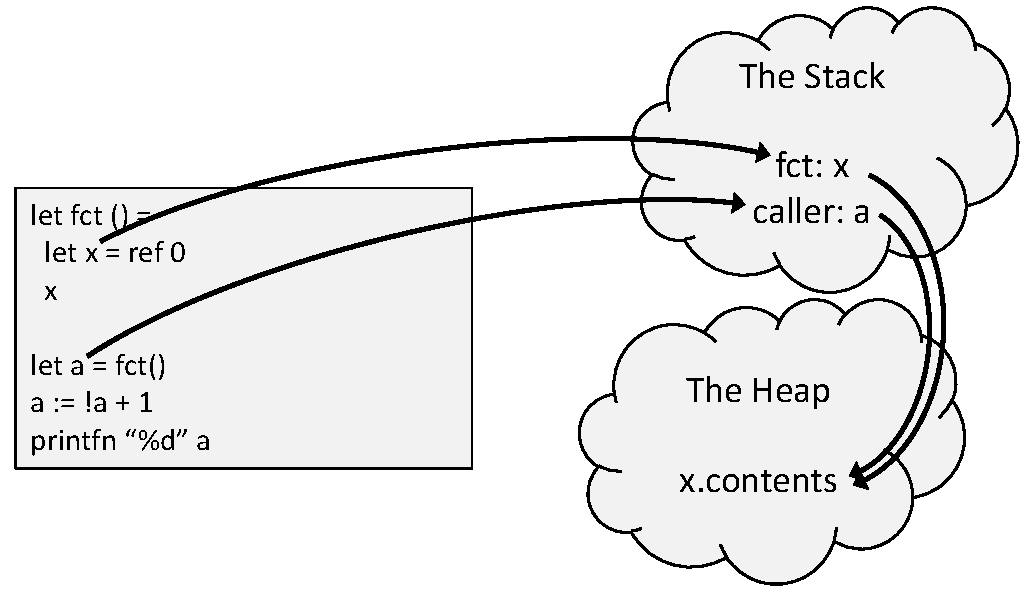
\includegraphics[width=0.6\textwidth]{ReferenceCells}
  \caption{A reference cell is a pointer to The Heap, and the content is not destroyed when its reference falls out of scope.}
  \label{fig:returningRefCells}
\end{figure}
%

Reference cells may cause \idx[side-effect]{side-effects}, where variable changes are performed across independent scopes. Some side-effects are useful, e.g., the \lstinline{printf} family changes the content of the screen, and the screen is outside the scope of the caller.  Another example of a useful side-effect is a counter shown in \Cref{refEncapsulation}.
%
\fs{refEncapsulation}{An increment function with a local state using a reference cell.}
%
Here \lstinline{incr} is an anonymous function with an internal state \lstinline{counter}. At first glance, it may be surprising that \lstinline{incr ()} does not return the value \lstinline{1} at every call. The reason is that the value of the \lstinline{incr} is the closure of the anonymous function \lstinline{fun () -> counter := ...}, which is 
\begin{equation}
  \text{\lstinline{incr}}: \left(\text{args}, \text{exp}, \text{env}\right)  = \big((), \left(\begin{subarray}{l}\displaystyle\text{\lstinline{counter := !counter + 1}}\\\displaystyle\text{\lstinline{!counter}}\end{subarray}\right), (\text{\lstinline{counter}}\rightarrow\text{\lstinline{ref 0}})\big).
\end{equation}
Thus, \lstinline{counter} is only initiated once at the initial binding, while every call of \lstinline{incr ()} updates its value on The Heap. Such a programming structure is called \idx{encapsulation}, since the \lstinline{counter} state has been encapsulated in the anonymous function, and the only way to access it is by calling the same anonymous function. In general, it is advisable to \advice{use encapsulation to hide implementation details irrelevant to the user of the code.}

The \lstinline{incr} example in \Cref{refEncapsulation} is an example of a useful side-effect. An example to be avoided is shown in \Cref{refSideEffect}.
%
\fs{refSideEffect}{Intertwining independent scopes is typically a bad idea.}
%
In the example, the function \lstinline{updateFactor} changes a variable in the scope of the function \lstinline{multiplyWithFactor}. The code style is prone to errors, since the computations are not local at the place of writing, i.e., in \lstinline{multiplyWithFactor}, and if \lstinline{updateFactor} were defined in a library, then the source code may not be available. Better style of programming is shown in \Cref{refWithoutSideEffect}.
%
\fs{refWithoutSideEffect}{A solution similar to \Cref{refSideEffect} without side-effects.}
%
Here, there can be no doubt in \lstinline{multiplyWithFactor} that the value of \lstinline{a} is changing. Side-effects do have their use, but should, in general, be avoided at almost all costs, and it is advised to \advice{minimize the use of side effects}.

Reference cells give rise to an effect called \idx{aliasing}, where two or more identifiers refer to the same data, as illustrated in \Cref{refCellAliasing}.
%
\fs{refCellAliasing}{Aliasing can cause surprising results and should be avoided.}
%
Here, \lstinline!a! is defined as a reference cell, and by defining \lstinline!b! to be equal to \lstinline!a!, we have created an alias. This can be very confusing since as the example shows, changing the value of \lstinline!b! causes \lstinline!a! to change as well. Aliasing is a variant of side-effects, and \advice{aliasing should be avoided at all costs}.

Since F\# version 4.0, the compiler has automatically converted mutable variables to reference cells, where needed.  E.g., \Cref{refEncapsulation} can be rewritten using a mutable variable, as shown in \Cref{mutableEncapsulation}.
% 
\fs{mutableEncapsulation}{Local mutable content can be indirectly accessed outside its scope.}
% 
Reference cells are preferred over mutable variables for encapsulation, in order to avoid confusion.

\section{Tuples}
\idx[tuple]{Tuples} are a direct extension of constants. They are immutable and have neither concatenations nor indexing operations. Tuples are unions of immutable types and have the following syntax:
%
\begin{verbatimwrite}{\ebnf/tuples.ebnf}
<*expr*>{*, <*expr*>*}
\end{verbatimwrite}
\syntax{\ebnf/tuples.ebnf}{Tuples are list of expressions separated by commas.}
%
Tuples are identified by the \lexeme{,} lexeme and often enclosed in parentheses, but that is not required. An example is a triple, also known as a 3-tuple, \lstinline!(2,true,"hello")!. In interactive mode, the type of tuples is demonstrated in \Cref{tuple}.
%
\fsOutput{tuple}{Tuple types are products of sets.}
%
The values \lstinline!2!, \lstinline!true!, and \lstinline!"hello"! are \idx[member]{members}, and the number of elements of a tuple is its \idx{length}. From the response of F\#, we see that the tuple is inferred to have the type \lstinline!int * bool * string!. The \lexeme{*} denotes the Cartesian product between sets.  Tuples can be products of any types and follow the lexical scope rules like value and function bindings. Notice also that a tuple may be printed as a single entity by the \lstinline!%A! %
placeholder. In the example we bound \lstinline!tp! to the tuple. The opposite is also possible, as demonstrated in \Cref{tupleDeconstruction}.
%
\fsOutput{tupleDeconstruction}{Definition of a tuple.}
%
In this example, a function is defined that takes 1 argument, a 3-tuple. If we wanted a function with 3 arguments, then the function binding should have been \lstinline{let deconstructNPrint a b c = ...}. The value binding \lstinline{let (a, b, c) = tp}, binds a tuple with 3 named members to a value, thus deconstructing it in terms of its members. This is called pattern matching and will be discussed in further details in \Cref{chap:patterns}. Since we used the \lstinline!\%A! placeholder in the \lstinline!printfn! function, the function can be called with 3-tuples of different types. F\# informs us that the tuple type is variable by writing \lstinline{'a * 'b * 'c}. The \lexeme{'} notation means that the type can be decided at run-time, see \Cref{sec:variableTypes} for more on variable types. 

Pairs or 2-tuples are so common that F\# includes two built-in functions,\idx[fst@\lstinline{fst}]{\keyword{fst}} and \idx[snd@\lstinline{snd}]{\keyword{snd}}, to extract the first and second element of a pair. This is demonstrated in \Cref{pair}.
%
\fs{pair}{Deconstruction of pairs with the built-in functions \keyword{fst} and \keyword{snd}.}
%

Tuples of equal lengths can be compared, and the  comparison is defined similarly to string comparison. Tuples of equal length are compared element by element. E.g., \lstinline!(1,2) = (1,3)! is false, while \lstinline!(1,2) = (1,2)! is true. The \lexeme{<>} operator is the boolean negation of the \lexeme{=} operator. For the \lexeme{<} , \lexeme{<=}, \lexeme{>}, and \lexeme{>=} operators, the strings are ordered lexicographically, such that \lstinline!('a', 'b', 'c') < ('a', 'b', 's') && ('a', 'b', 's') <  ('c', 'o', 's')! is true, that is, the \lexeme{<} operator on two tuples is true if and only if the left operand should come before the right when sorting alphabetically. See \Cref{tupleCompare} for an example.
%
\fs{tupleCompare}{Tuples comparison is similar to string comparison.}
%
The algorithm for deciding the boolean value of \lstinline!(a1, a2) < (b1, b2)! is as follows: we start by examining the first elements, and if \lstinline!a1! and \lstinline!b1! are different, then the result of \lstinline!(a1, a2) < (b1, b2)! is equal to the result of \lstinline!a1 < b1!. If \lstinline!a1! and \lstinline!b1! are equal, then we move on to the next letter and repeat the investigation. The \lexeme{<=}, \lexeme{>}, and \lexeme{>=} operators are defined similarly.

Binding tuples to mutables does not make the tuple mutable. This is demonstrated in \Cref{tupleOfMutables}.
%
\fs{tupleOfMutables}{A mutable changes value, but the tuple defined by it does not refer to the new value.}
%
However, it is possible to define a mutable variable of type tuple such that new tuple values can be assigned to it, as shown in \Cref{mutableTuple}.
%
\fs{mutableTuple}{A mutable tuple can be assigned a new value.}
%
Mutable tuples are value types, meaning that binding to new names makes copies, not aliases, as demonstrated in \Cref{mutableTupleValue}.
%
\fs{mutableTupleValue}{A mutable tuple is a value type.}
%
The use of tuples shortens code and highlights semantic content at a higher level, e.g., instead of focusing on the elements, tuples focus on their union. While this may look elegant and short there is the risk of \idx{obfuscation}, i.e., writing compact code that is difficult to read, where an unprepared reader of the code may not easily understand the computation nor appreciate its elegance without an accompanying explanation.  Hence, \advice{always keep an eye out for compact and concise ways to write code, but never at the expense of readability.}

%%% Local Variables:
%%% TeX-master: "fsharpNotes"
%%% End:

